\section{Prototype}
\label{section:prototyping}

Om te controleren of de detectiemethode die geselecteerd is in hoofdstuk~\ref{section:detection}
gebruikt kan worden om mogelijk op een tremor te reageren,
zal er een prototype gemaakt worden.
Dit hoofdstuk bevat een beschrijving van de keuzes die zijn gemaakt tijdens het maken van dit prototype;
hiermee beantwoordt het deels de vraag: Hoe kan de data die uit een detectie komt worden gebruikt?

\subsection{Wat wordt er gemaakt?}

De gekozen detectiemethode uit hoofdstuk~\ref{section:detection} is de EMG.
Om de bruikbaarheid van deze methode te testen, zal er een prototype worden gemaakt.
Gezien het doel van het onderzoek is om te mogelijkheid te verifiëren, ligt de focus niet op perfectie.
De richting zal vooral in theorie zijn, met mogelijke vervolgstappen in hoofdstuk~\ref{section:application}.

\subsection{Wat zijn bestaande implementaties?}

Voordat er gekeken wordt naar het implementeren van eigen EMG,
zal er kort worden gekeken naar de manieren waarop een EMG geïmplementeerd kan worden.
Het gaat daarbij vooral over soorten implementaties, niet specifieke implementaties. 
Een EMG kan namelijk op verschillende manieren worden gedaan.
Er wordt onderscheid gemaakt tussen drie soorten implementaties en twee systemen \cite{gohel2020}.

Desktop EMG-machines worden vooral gebruikt in een kliniek, ze zijn groot en accuraat;
deze zijn in kleiner draagbaar formaat te verkrijgen als Portable EMG's \cite{neurostyle2021,cadwell2023}.
Een portable EMG is meestal een kleiner apparaat dat bediend wordt door middel van een laptop,
ze worden vooral gebruikt tijdens onderzoeken \cite{neurostyle2021}.
In Figuur~\ref{figure:emgmachine} zijn deze EMG-vormen van CADWELL te zien \cite{cadwell2023}.

\begin{center}
    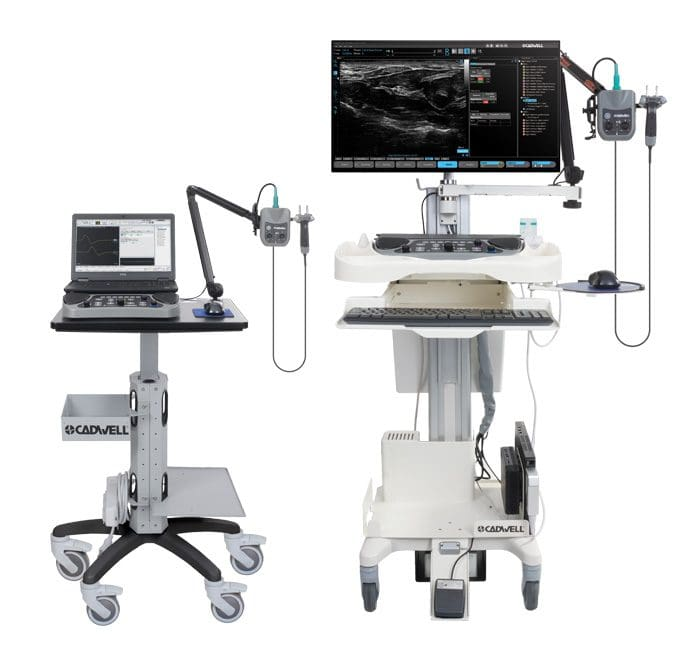
\includegraphics[width=0.4\textwidth]{./graphics/img-emgcarts.jpg}
    \captionof{figure}{Portable en Desktop EMG}
    \label{figure:emgmachine}
\end{center}

Een horloge variant van een EMG machine is verkrijgbaar om langdurig, of bij specifieke activiteiten, 
spieractiviteit te kunnen registreren en analyseren \cite{sips2024,activinsights2022}. 
Figuur~\ref{figure:emgwatch} toont de GENEActiv: Raw Data Accelerometer \cite{activinsights2022}.

\begin{center}
    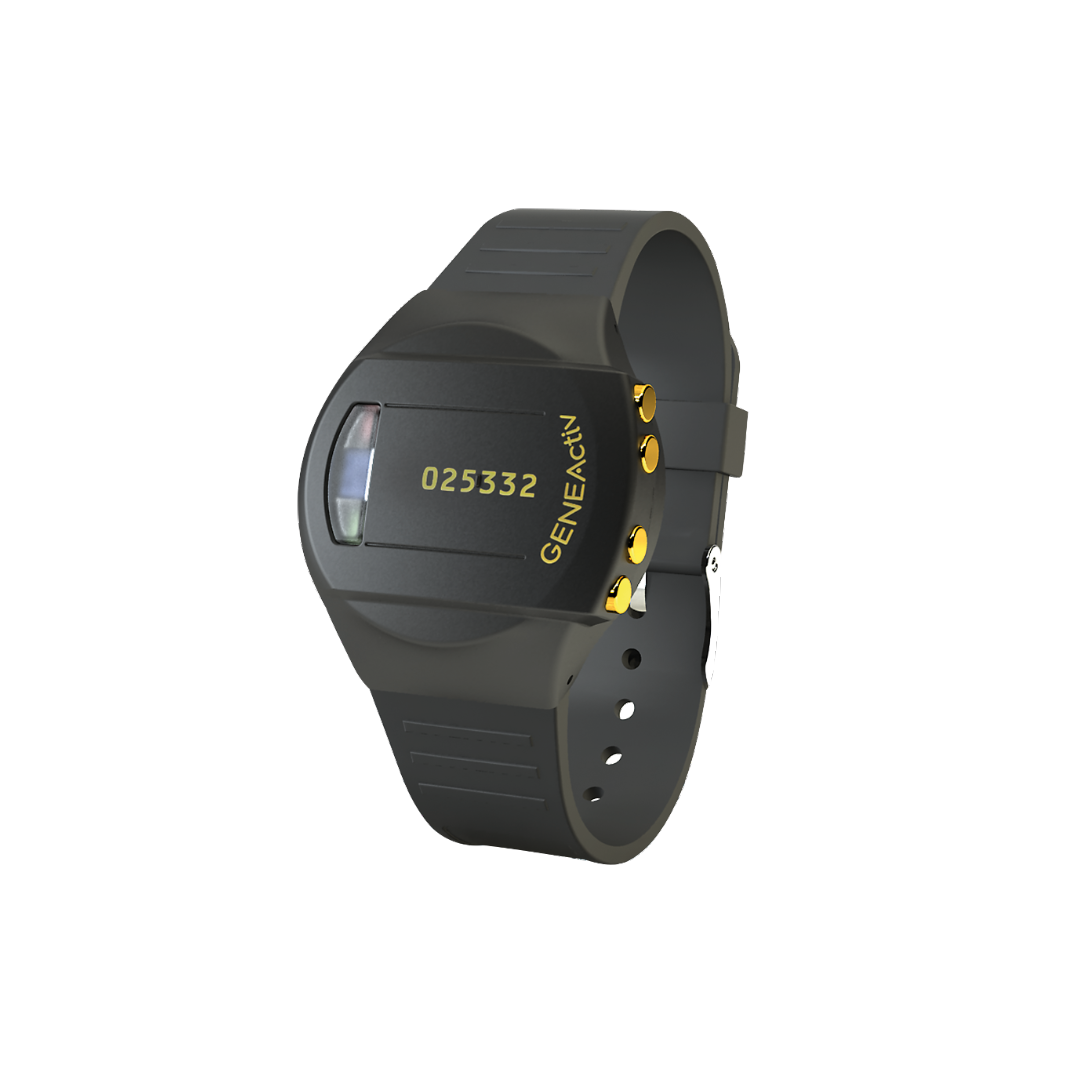
\includegraphics[width=0.4\textwidth]{./graphics/img-emgwatch.png}
    \captionof{figure}{GENEActiv: Raw Data Accelerometer}
    \label{figure:emgwatch}
\end{center}

Onder de system vallen draadloze systemen en geïntegreerde systemen \cite{gohel2020}.
De systemen vallen buiten de scope van dit onderzoek.

\subsection{Wat is er gebruikt?}

Voor de ontwikkeling van het prototype is er gebruik gemaakt van een Arduino Uno R3.
Dit is het hart van het prototype en verzorgt de verwerking van de gegevens.
Om de gegevens van de elektroden te kunnen lezen, wordt er gebruik gemaakt van een spiersensor.
De sensor set de signalen van de elektroden om in gegevens die gebruikt kunnen worden door de Arduino.
Een breadboard wordt gebruikt om alles met elkaar te verbinden \cite{emg2021}.

\begin{center}
    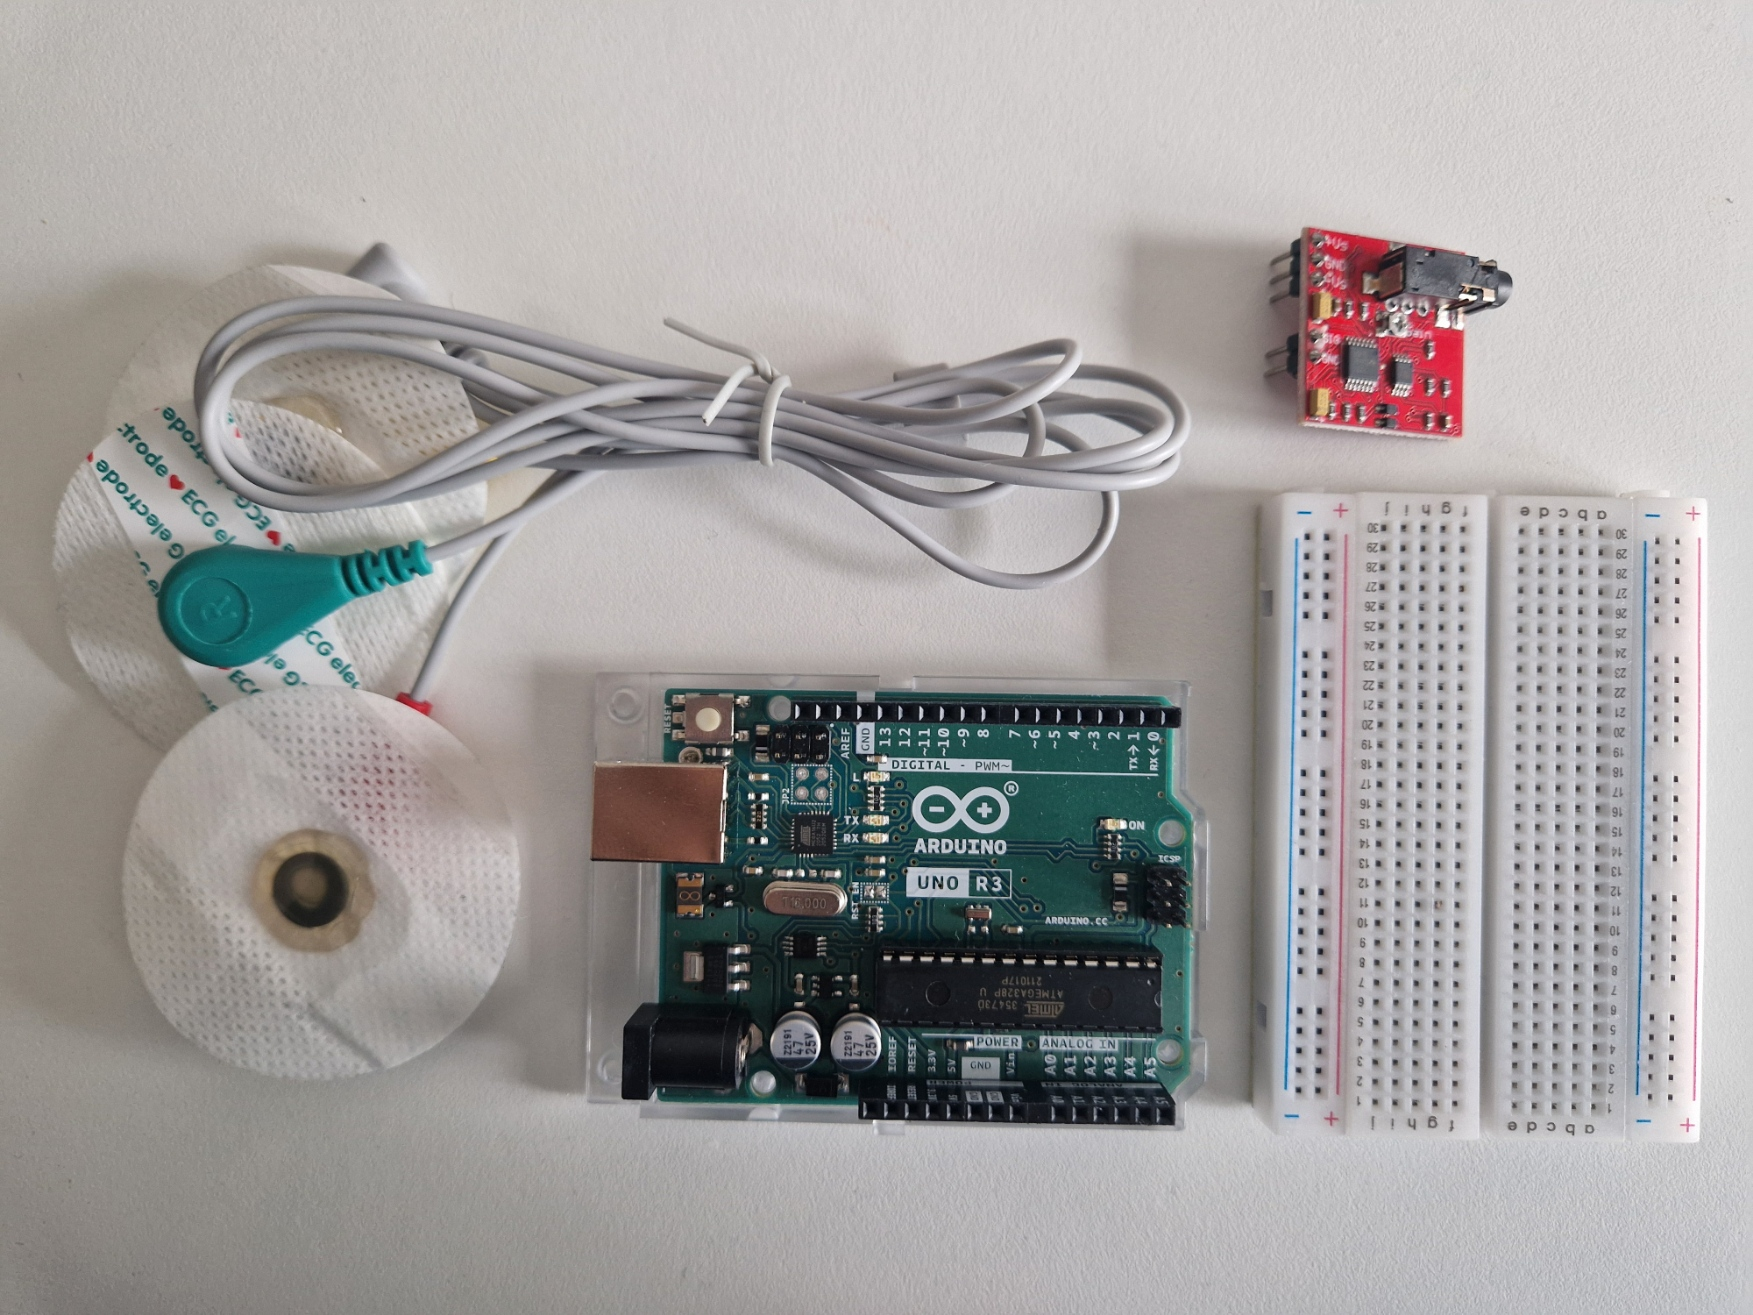
\includegraphics[width=0.4\textwidth]{./graphics/img-components.jpg}
    \captionof{figure}{Onderdelen van het Prototype: Electroden, Spiersensor, Arduino Uno R3 \& Breadboard}
    \label{figure:components}
\end{center}

\subsection{Hoe is het gemaakt?}

De spiersensor communiceert met de elektroden door middel van een 3,5mm kabel.
De sensor zet de geluiden die het hoort om in waardes die gelezen kunnen worden door de Arduino.
Als stroombron worden hiervoor twee 9-volt batterijen gebruikt.
De signaal-pin wordt aangesloten aan een analoge input van de Arduino \cite{emg2021}.
Dit is als schema te zien in Figuur~\ref{figure:arduino}.

\begin{center}
    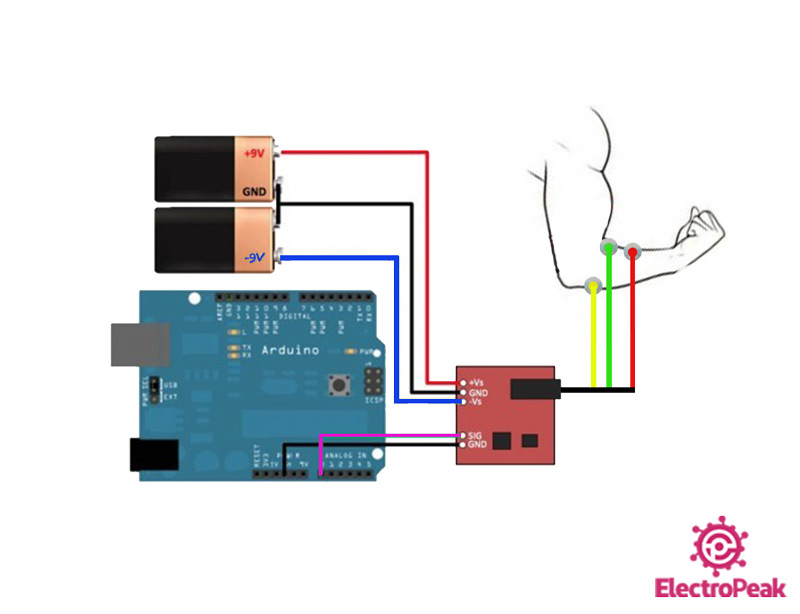
\includegraphics[width=0.4\textwidth]{./graphics/graph-arduino.jpg}
    \captionof{figure}{Diagram Prototype}
    \label{figure:arduino}
\end{center}

Om dit te doen met de fysieke hardware, is er begonnen met een breadboard.
Op deze manier zijn de verschillende stappen makkelijker te documenteren,
waarbij de acties beter zichtbaar zijn.
De spiersensor wordt in het breadboard geprikt, dit is te zien in Figuur~\ref{figure:stepa}.

Vervolgens worden de verbindingen gelegd.
Voor dit prototype, zal de 5-volt-lijn van de Arduino worden gebruikt.
Het signaal zal zwakker zijn, maar het verwijderd de benodigdheid voor de twee batterijen.
De witte draad verbindt de 5-volt-lijn met de spiersensor; de twee zwarte draden doen dit voor grondlijn.
De oranje draad wordt gebruikt voor het signaal, de bruine voor de grondlijn voor deze verbinding.
Voor het overzicht, 
zijn 5-volt-lijn en de grondlijn verwijderd voor het nemen van de foto in Figuur~\ref{figure:stepb}.

De code die is geschreven voor het project is makkelijk te begrijpen.
De Arduino wordt ingesteld om te communiceren via seriële poort 9600,
waarna de gegevens die verkregen worden van de spiersensor worden afgedrukt \cite{emg2021}.
De code is terug te vinden op GitHub via \url{https://github.com/Jimmaphy/tremor-detection}.
Het resultaat van de code is een lange lijst aan getallen die de gegevens van de spiersensor voorstellen.
Dit resultaat is terug te zien in Figuur~\ref{figure:output} van de volgende paragraaf.
De mogelijke toepassing van deze output wordt besproken in hoofdstuk~\ref{section:application}.

\begin{center}
    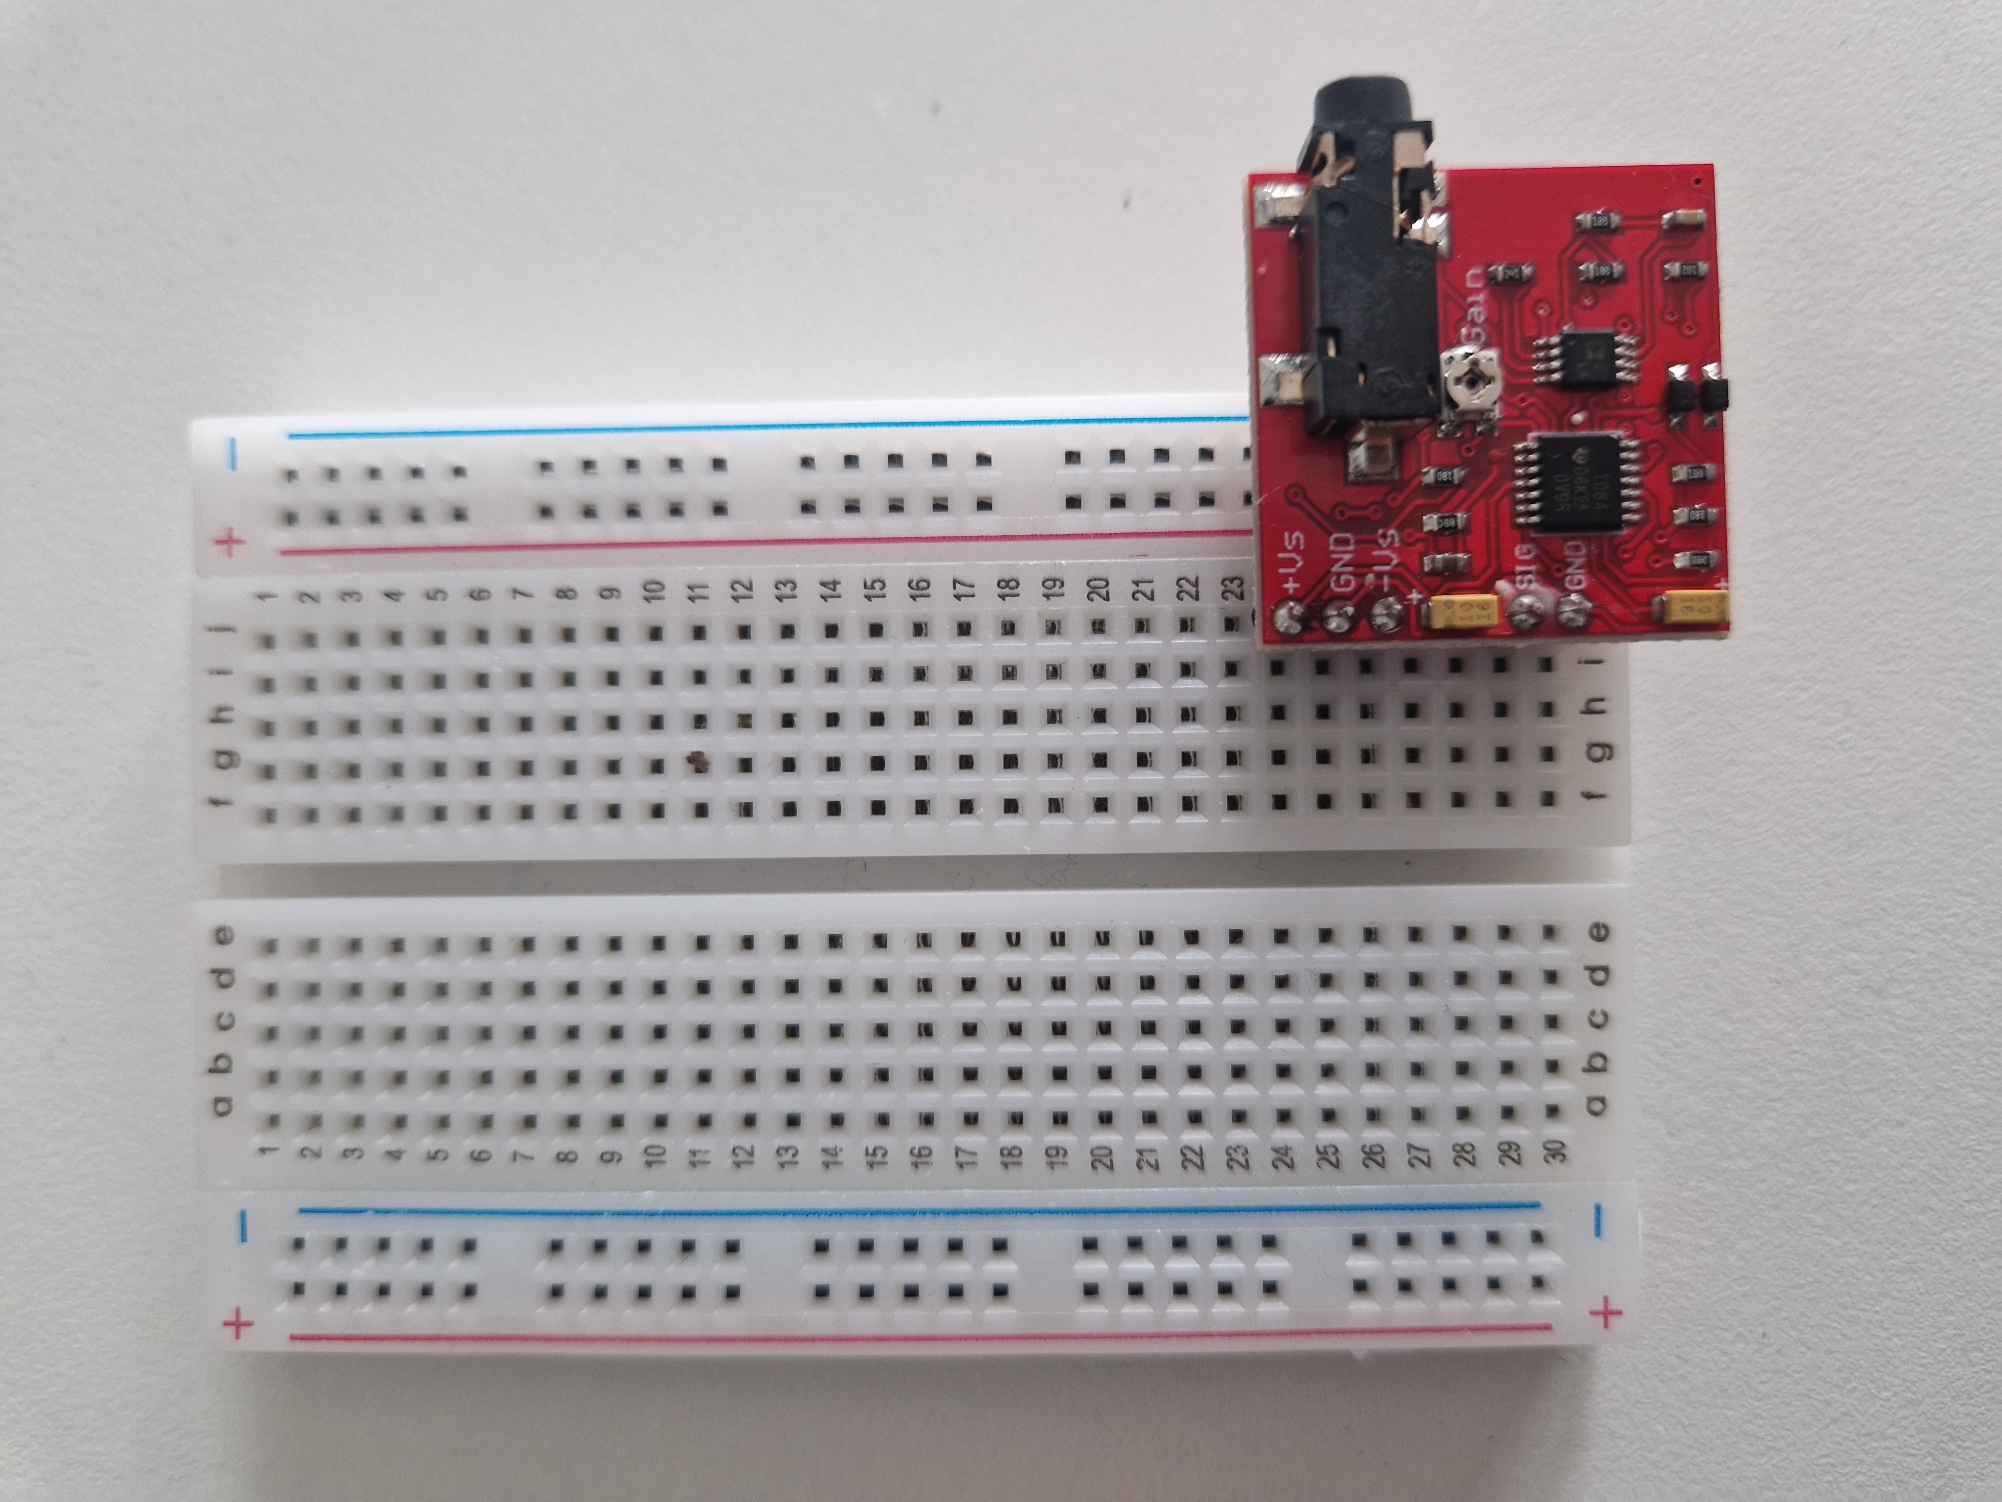
\includegraphics[width=0.4\textwidth]{./graphics/img-step1.jpg}
    \captionof{figure}{Spiersensor in een Breadboard}
    \label{figure:stepa}
\end{center}

\begin{center}
    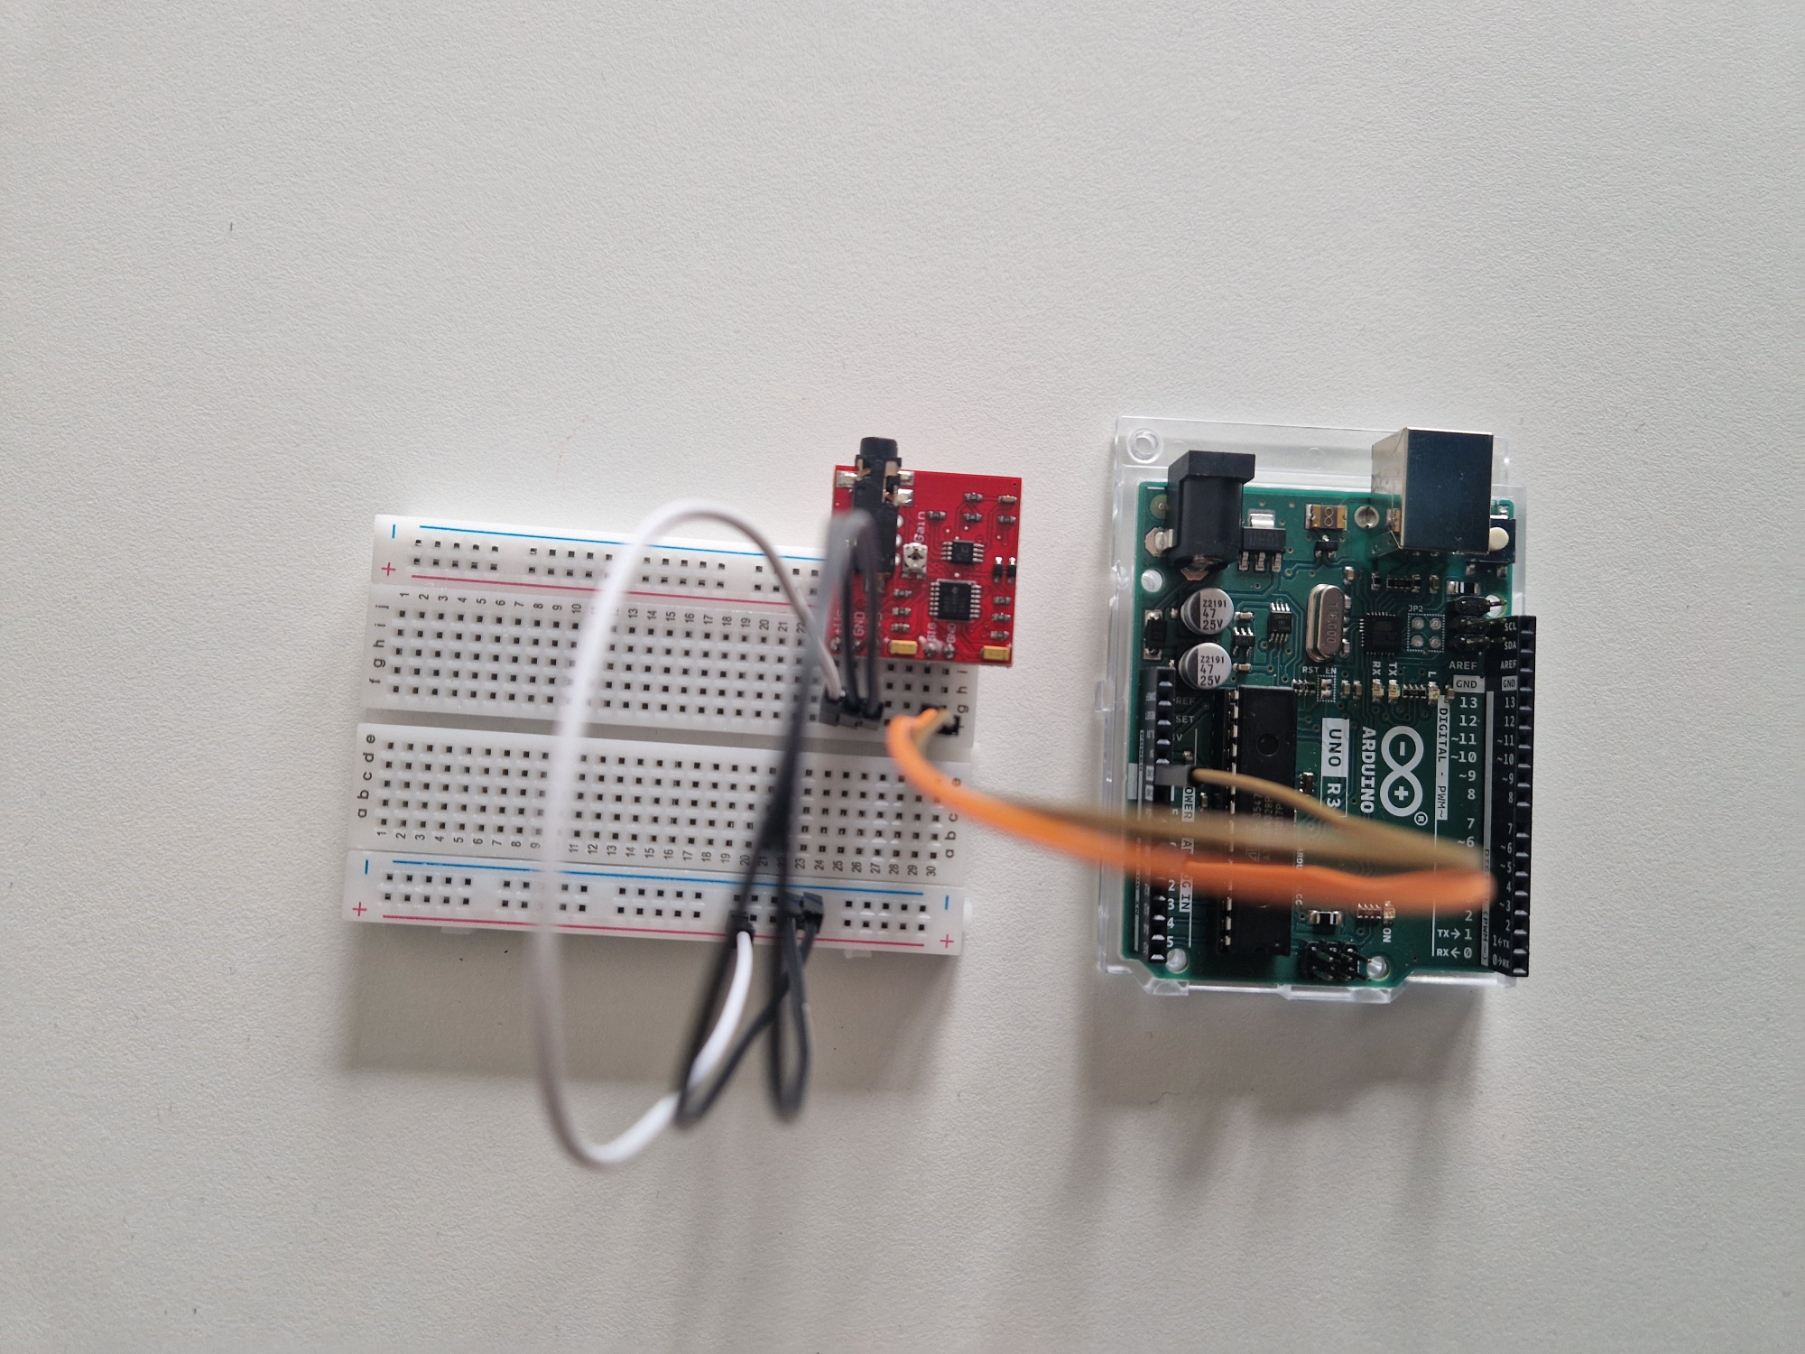
\includegraphics[width=0.4\textwidth]{./graphics/img-step2.jpg}
    \captionof{figure}{Arduino Verbonden met de Sensor}
    \label{figure:stepb}
\end{center}

\subsection{Wat kan het?}

Om het prototype correct te gebruiken, zijn twee 9-volt batterijen nodig.
Deze zijn tijdens het onderzoek niet gebruikt.
Het signaal veranderde echter netjes op het moment dat er activiteit was in de spieren,
maar het verschil was bijna niet te zien.
Een voorbeeld van de data met juiste stroombron is te zien in Figuur~\ref{figure:screenshot}, 
de gemeten data in Figuur~\ref{figure:output}.

\begin{center}
    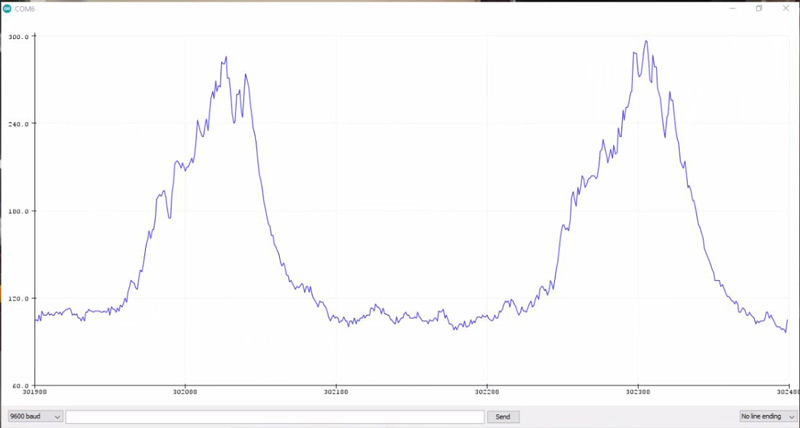
\includegraphics[width=0.4\textwidth]{./graphics/screenshot-emg.jpg}
    \captionof{figure}{Output Spiersensor als Grafiek}
    \label{figure:screenshot}
\end{center}

\begin{center}
    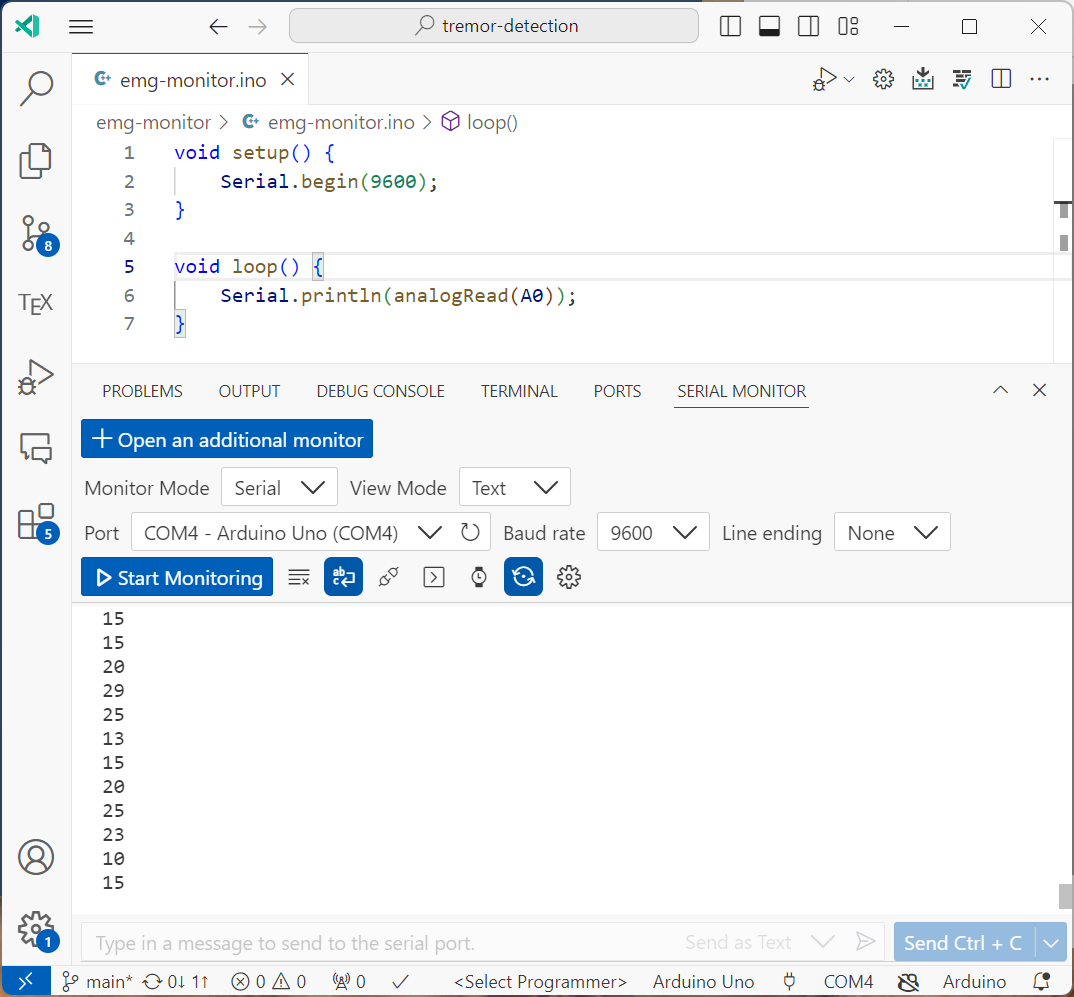
\includegraphics[width=0.4\textwidth]{./graphics/screenshot-serial.png}
    \captionof{figure}{Output Spiersensor Prototype}
    \label{figure:output}
\end{center}

